\documentclass[11pt]{utalcaDoc}
\usepackage{alltt}
\usepackage{underscore}
\usepackage[utf8]{inputenc}
\usepackage[activeacute,spanish]{babel}
\usepackage{verbatim}
\usepackage[pdftex]{graphicx}
\usepackage{ae}
\usepackage{amsmath}
\usepackage{amsfonts}
\usepackage{pdflscape}
\usepackage{inconsolata}
\usepackage{url}
\usepackage{listings}
% \usepackage{placeins}
\usepackage[section]{placeins}

\title{{\bf Administración de Redes de Computadores}\\ Laboratorio 4}

\author{Erik Regla\\ eregla09@alumnos.utalca.cl}
\date{\today}
\lstset{language=SH, 
		basicstyle=\ttfamily\tiny, 
		showspaces=false, 
		numbers=left, 
		breaklines=true,
		frame=shadowbox
		}

\begin{document}
\maketitle

\section{Cree un diagrama con la misma forma, adjunte cada mac a los switch, agregue un pc a cada switch, identifique el switch root, haga ping true entre 2 pc, elimine o desactive la ruta que este est\'a usando. ¿Qu\'e sucede al eliminar la ruta usada? ¿Explique qu\'e pas\'o? evidencie todo el proceso.}


\begin{figure}[!ht]
  \centering

\includegraphics[scale=.3]{1} 
  \caption{Antes de cortar el enlace}
  \label{FIGURE:1}
\end{figure}

\begin{figure}[!ht]
  \centering
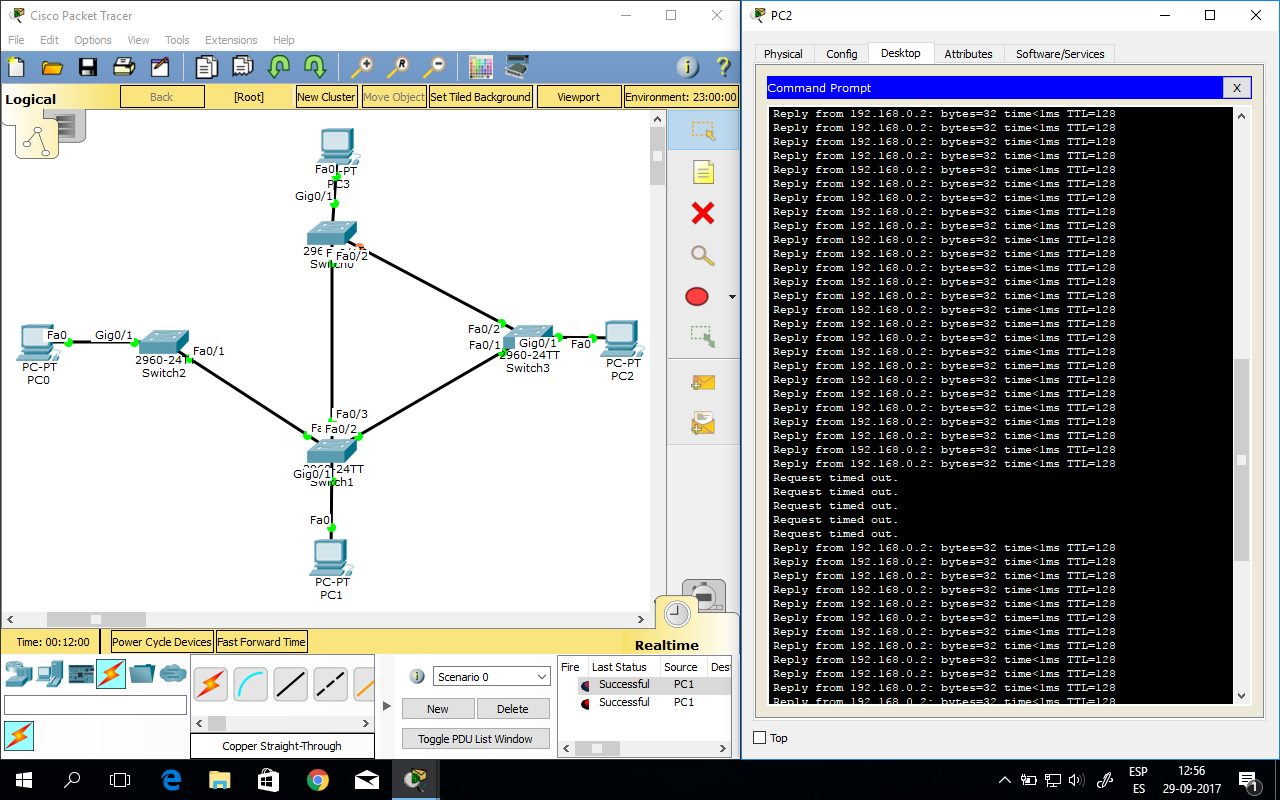
\includegraphics[scale=.3]{2} 
  \caption{Después de cortar el enlace}
  \label{FIGURE:2}
\end{figure}

La conexión se pierde mientras se resuelve un nuevo MST. Una vez resuelto la conexión se reestablece.


\section{Cambie el switch root (sin cambiar los switch), y vuelva a repetir los pasos de 1, ¿En qu\'e afecta el cambiar el root? (Use comando spanning-tree vlan 1 root primary)}


\begin{figure}[!ht]
  \centering
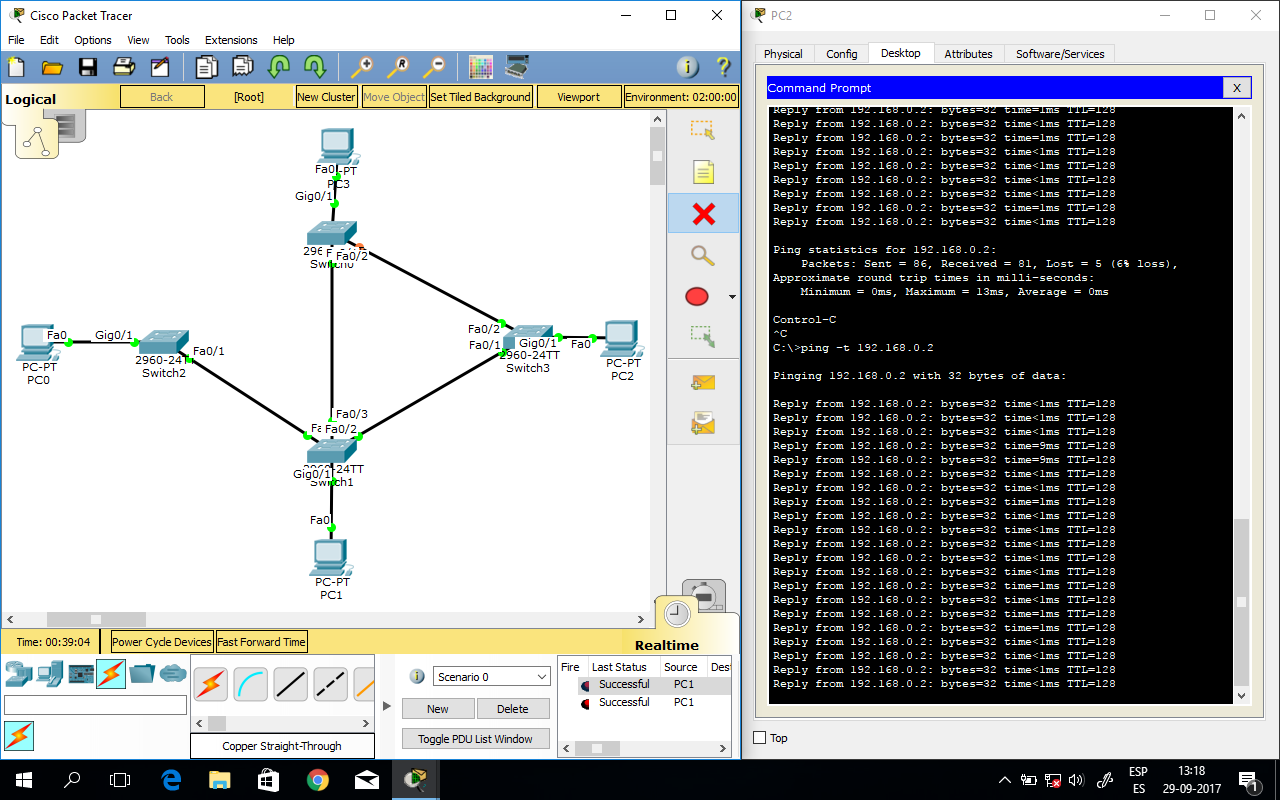
\includegraphics[scale=.3]{3} 
  \caption{Cortando el enlace}
  \label{FIGURE:3}
\end{figure}

Nada. Dado que el el switch 2 fue designado como el puente raiz, el MST extiende directamente desde ese nodo a todos los demás, desactivando el puente entre s2 y s3 y s0 con s1. Como fue cortado una vía que no estaba en uso, no pasó nada.


\section{Concluya sobre el trabajo realizado. ¿Qu\'e ventajas y desventajas se perciben en Spanning Tree Protocol? ¿Es eficiente este protocolo?}

La única desventaja a mi parecer es que uno no tiene control absoluto de como se resuelve el arbol, lo cual en ciertas topologías puede ser un problema. La ventaja es la misma, al no tener control sobre el, no es necesario monitorear constantemente, eliminando la intervención humana durante el proceso.

De que sea eficiente o no ese es otro problema. Dependerá directamente de las condiciones en las cuales se despliegue la solución. Si los enlaces estan predispuestos a dañarse sin patrón alguno es buena idea dejarlo como está. De otro modo es mejor sugerir raices y establecer fallbacks en vez de dejar todo automático (para así no sufrir outages debido a la resolución del MST).


\section{Haciendo uso de Packet Tracer, se solicita crear una red, que conste con el diagrama anterior, conecte 1 computador a cada switch de abajo(a), 1 router a cada switch de arriba, luego conecte estos 2 router a otro router, para as\'i ponerle un dispositivo final(b)}


\begin{figure}[!ht]
  \centering
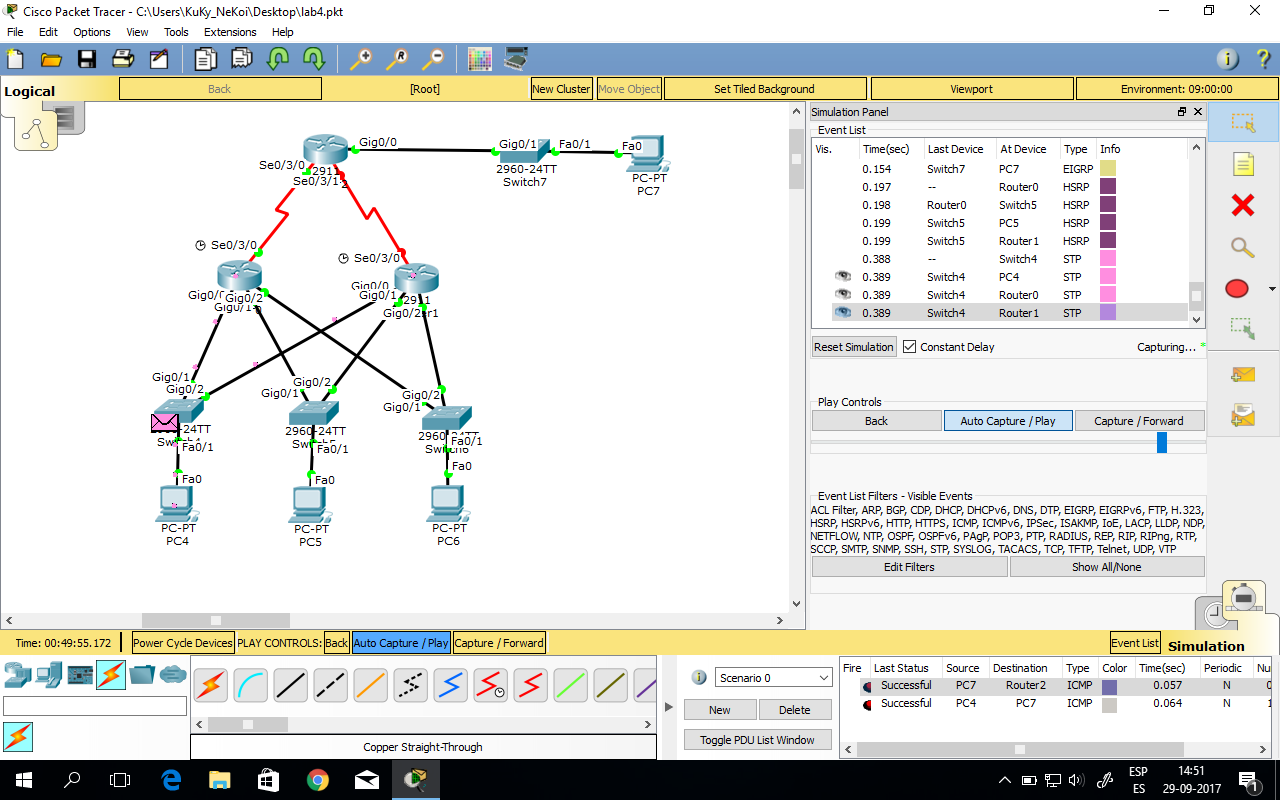
\includegraphics[scale=.3]{4} 
  \caption{Red creada}
  \label{FIGURE:4}
\end{figure}



\section{Cree varias redes para que los equipos tengan comunicaci\'on entre s\'i, compruebe que haya conexi\'on entre ellos(ping). Configure ambos router con la misma puerta de enlace y as\'ignele m\'as prioridad a uno (standby 1 priority XX).}


\begin{figure}[!ht]
\begin{lstlisting}
  ! router 0
  enable
      configure terminal
          interface GigabitEthernet0/0
              ip address 192.168.1.2 255.255.255.0
              standby ip 192.168.1.1
              standby preempt
              no shutdown
          exit
          interface GigabitEthernet0/1
              ip address 192.168.2.2 255.255.255.0
              standby ip 192.168.2.1
              standby preempt
              no shutdown
          exit
          interface GigabitEthernet0/2
              ip address 192.168.3.2 255.255.255.0
              standby ip 192.168.3.1
              standby preempt
              no shutdown
          exit
          interface Serial0/3/0
              ip address 10.0.0.2 255.0.0.0
              standby ip 10.0.0.1
              standby preempt
              clock rate 2000000
              no shutdown 
          exit
          router eigrp 10
              network 192.168.1.0 255.255.255.0
              network 192.168.2.0 255.255.255.0
              network 192.168.3.0 255.255.255.0
              network 10.0.0.0 255.0.0.0
          exit
      exit
      copy running-config startup-config
      startup-config 
  exit
\end{lstlisting}
\label{FIG:ROUTER0}
\caption{Scripting para configuración de Router0}
\end{figure}

\begin{figure}[!ht]
\begin{lstlisting}
  ! router 1
  enable
      configure terminal
          interface GigabitEthernet0/0
              ip address 192.168.1.3 255.255.255.0
              standby ip 192.168.1.1
              standby priority 99
              no shutdown
          exit
          interface GigabitEthernet0/1
              ip address 192.168.2.3 255.255.255.0
              standby ip 192.168.2.1
              standby priority 99
              no shutdown
          exit
          interface GigabitEthernet0/2
              ip address 192.168.3.3 255.255.255.0
              standby ip 192.168.3.1
              standby priority 99
              no shutdown
          exit
          interface Serial0/3/0
              ip address 10.0.0.3 255.0.0.0
              standby ip 10.0.0.1
              standby preempt
              clock rate 2000000
              no shutdown 
          exit
          router eigrp 10
              network 192.168.1.0 255.255.255.0
              network 192.168.2.0 255.255.255.0
              network 192.168.3.0 255.255.255.0
              network 10.0.0.0 255.0.0.0
          exit
      exit
      copy running-config startup-config
      startup-config 
  exit
\end{lstlisting}
\label{FIG:ROUTER1}
\caption{Scripting para configuración de Router1}
\end{figure}

\begin{figure}[!ht]
\begin{lstlisting}
  ! router 2
  enable
      configure terminal
          interface GigabitEthernet0/0
              ip address 192.168.4.1 255.255.255.0
              no shutdown 
          exit
          interface Serial0/3/0
              ip address 10.0.0.4 255.0.0.0
              clock rate 2000000
              no shutdown 
          exit
          interface Serial0/3/1
              ip address 10.0.0.5 255.0.0.0
              clock rate 2000000
              no shutdown 
          exit
  
          router eigrp 10
              network 192.168.4.0 255.255.255.0
              network 10.0.0.0 255.0.0.0
          exit
      exit
      copy running-config startup-config
      startup-config 
  exit
\end{lstlisting}
\label{FIG:ROUTER2}
\caption{Scripting para configuración de Router2}
\end{figure}
      
\section{Concluya sobre el trabajo realizado. ¿Qu\'e ventajas y desventajas se perciben en usar HSRP?, ¿Qu\'e tan f\'acil/dif\'icil resultar\'ia agregar otro router?}

Como desventajas es una mayor configuración, dado que hay que tener registro de las IPs virtuales involucradas y de las usadas como mirror. Respecto a las ventajas tenemos redundancia de conexión (no confundir con agregación de enlace), por lo que nuestra red es más robusta (en el sentido que si se cae un enlace solo hay un downtime menor sin necesidad de intervención humana.)

No es más dificil agregar otro router si se considera tener respaldo de la configuración.

\end{document}